\documentclass[../main.tex]{subfiles}

\begin{document}
	\section{Turning Effect of Forces}
	\begin{preamb}
		Objects do not only move in a straight line, they can also move in curves and circles and all kinds of funny shapes. In this chapter we will explore how we can make an object turn by applying a force.
	\end{preamb}

	\subsection{Moment}
		\pdef{Moment}{The moment of a force is the product of the force \(F\) and the perpendicular distance from the pivot to the line of action of the force \(r\) \[\mathrm{moment} = r \times F\] The SI unit of moment is newton metre [\si{\newton \metre}].}
		
		\begin{center}
			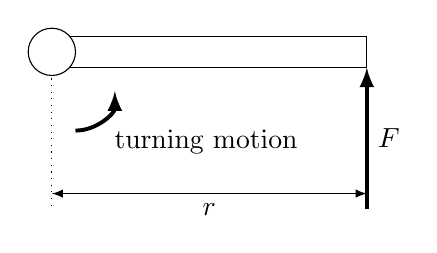
\begin{tikzpicture}
				\draw (0,-0.2) rectangle (4,0.2);
				\draw [dotted] (0,0) -- (0,-2);
				\filldraw [fill=white, draw=black] (0,0) circle (3mm);
				\draw [line width=0.5mm, -latex] (4,-2) -- (4,-0.2) node[pos=0.5, anchor=west] {\(F\)};
				\draw [latex-latex] (0,-1.8) -- (4,-1.8) node[pos=0.5, anchor=north] {\(r\)};
				\draw (0.3,-1)[line width=0.5mm, -latex] arc (-90:0:0.5) node[pos=0.5, anchor=north west] {turning motion};
			\end{tikzpicture}
		\end{center}
	
		\pdef{Principle of Moments}{The principle of moments states that when a body is in equilibrium, the sum of clockwise moments about a pivot is equal to the sum of anticlockwise moments about the same pivot..}
		
	\subsection{Centre of Gravity}
		\pdef{Centre of Gravity}{The centre of gravity, or centre of mass, is a point where the weight of an object seems to be acting on. The centre of gravity can lie outside an object.}
		
	\subsection{Stability}
	
		\pdef{Stability}{The stability of an object is a measure of its ability to return to its original position after it is s lightly displaced.}
	
		An object can be in stable, unstable, or neutral equilibrium.
		\begin{center}
		\begin{tabularx}{0.85\linewidth}{X|XXX}
			\hline \hline
			Type of equilibrium & Stable & Unstable & Neutral \\
			\hline
			Centre of gravity & Low & High & \\
			Base area & Large & Narrow & A line of contact points with surface \\
			Slight displacement & Return to equilibrium & Topple over & Stay in new position \\
			\hline \hline
		\end{tabularx}
		\end{center}
	
		An object's stability can be increased by lowering the height of the centre of gravity, or increasing the base area of the object.
\end{document}